\documentclass[conference]{IEEEtran}
\IEEEoverridecommandlockouts

\usepackage[utf8]{inputenc}
\usepackage[T1]{fontenc}
\usepackage[shorthands=off, turkish]{babel}
\usepackage{cite}
\usepackage{amsmath,amssymb,amsfonts}
\usepackage{graphicx}
\graphicspath{{figures/}{./}}
\usepackage{booktabs}
\usepackage{tabularx}
\usepackage{array}
\usepackage{xcolor}
\usepackage{hyperref}

\hypersetup{
    colorlinks=true,
    linkcolor=blue!70!black,
    citecolor=blue!70!black,
    urlcolor=blue!70!black
}

\begin{document}

\title{Önceden Eğitilmiş Türkçe Modellerle İnce Ayar (Fine-Tuning) Tabanlı Chatbot Geliştirme ve Seq2Seq Karşılaştırmalı Başarım Analizi\\
{\large\textit{Nihai Proje Raporu (Final Paper) --- Deep Learning (2026--2027)}}}

\author{\IEEEauthorblockN{Seyit Ali Arslan}
\IEEEauthorblockA{\textit{Yapay Zeka ve Veri Mühendisliği Bölümü} \\
\textit{Atatürk Üniversitesi}\\
Erzurum, Türkiye \\
Öğrenci No: 240711024 \\
GitHub: \url{https://github.com/sytali0/turkish-transformer-chatbot}}
}

\maketitle

\begin{abstract}
Doğal Dil İşleme (NLP) alanında Türkçe gibi sondan eklemeli (agglutinative) ve zengin morfolojik yapıya sahip dillerde akıcı, mantıksal tutarlılığı yüksek ve bağlamı koruyan diyalog sistemleri geliştirmek önemli bir araştırma problemidir. Bu çalışmada, sıfırdan büyük dil modeli eğitmenin getirdiği aşırı hesaplama maliyeti yerine, açık kaynaklı önceden eğitilmiş bir Türkçe Transformer modeli (\texttt{Turkish-GPT-2}, $\sim$124.4M parametre) 50.000 filtrelenmiş Türkçe diyalog çifti üzerinde hem Tam İnce Ayar (Full Fine-Tuning) hem de Parametre Verimli İnce Ayar (LoRA / PEFT) yöntemleriyle adapte edilmiştir. Geliştirilen Transformer modelleri, sıfırdan eğitilen 2 katmanlı Çift Yönlü Seq2Seq Bi-LSTM + Bahdanau Attention temel (Baseline) mimarisiyle doğrulama kaybı (Validation Loss), Perplexity (PPL), BLEU-1/2, ROUGE-1/L, çıkarım gecikmesi (Inference Latency) ve niteliksel insan değerlendirmesi (Human Evaluation) ölçütleri üzerinden karşılaştırılmıştır. Deneysel bulgular; Full Fine-Tuning modelinin Perplexity değerini 1328.04'ten 32.03'e (41.5 kat iyileşme) düşürdüğünü, LoRA modelinin ise parametrelerin yalnızca \%1.29'unu (1.62M parametre) güncelleyerek eğitim süresini \%28.7 kısalttığını ve 56.50 Perplexity ile Baseline modele kıyasla 23.5 kat daha yüksek dil tutarlılığı sağladığını kanıtlamaktadır.
\end{abstract}

\begin{IEEEkeywords}
Transformer, Fine-Tuning, LoRA, PEFT, Transfer Learning, Türkçe Doğal Dil İşleme, Chatbot, Seq2Seq Bi-LSTM, Bahdanau Attention, Perplexity, BLEU, ROUGE.
\end{IEEEkeywords}

\section{Giriş ve Problem Tanımı}
Doğal Dil İşleme (NLP) alanında Türkçe gibi sondan eklemeli (\textit{agglutinative}) ve zengin morfolojik yapıya sahip dillerde akıcı, mantıksal tutarlılığı olan ve bağlamı koruyan diyalog sistemleri kurmak önemli bir zorluktur. Kelime köklerine eklenen yapım ve çekim ekleri, yüzeysel kelime dağarcığının üstel olarak büyümesine ve kelime dışı (\textit{Out-of-Vocabulary -- OOV}) sorununa yol açmaktadır \cite{sennrich2016}.

Geleneksel Yinelemeli Sinir Ağı (RNN/LSTM) tabanlı diziden-diziye (\textit{Sequence-to-Sequence -- Seq2Seq}) mimariler, sıralı veri işleme yapıları nedeniyle uzun dizilerde bağlamı kaybetmekte (\textit{darboğaz / bottleneck problemi}) ve donanım kaynaklarını paralel işleyememektedir \cite{bahdanau2014}. Büyük dil modellerini sıfırdan eğitmek ise devasa veri kümesi ve yüksek hesaplama gücü gerektirdiğinden, bu çalışmada önceden eğitilmiş (\textit{Pre-trained}) açık kaynaklı Transformer ağırlıkları kullanılmış; model hedeflenen Türkçe diyalog verisi üzerinde hem tam ince ayar (\textit{Full Fine-Tuning}) hem de düşük dereceli adaptasyon (\textit{Low-Rank Adaptation -- LoRA}) süreçlerinden geçirilmiştir \cite{vaswani2017, radford2019, hu2022lora}.

\section{Motivasyon}
Önceden genel Türkçe metinler üzerinde eğitilmiş ağırlıkları transfer etmek (\textit{Transfer Learning}), eğitim süresini ve donanım ihtiyacını ciddi oranda düşürürken modelin dil bilgisi ve anlamsal kavrayışını korur. Projenin temel motivasyonu; sıfırdan eğitilen klasik bir 2 katmanlı Seq2Seq Bi-LSTM + Bahdanau Attention modeli, tam ince ayar yapılmış \texttt{Turkish-GPT-2} modeli ve parametre verimli LoRA / PEFT ile ince ayar yapılmış \texttt{Turkish-GPT-2} modelinin Türkçe diyalog bağlamındaki başarımını ve donanım verimliliğini somut, ölçülebilir metriklerle karşılaştırmaktır.

\section{Veri Kümesi ve Keşifsel Veri Analizi (EDA)}
Hugging Face üzerindeki açık erişimli Türkçe diyalog kaynaklarından (\texttt{Ba2han/Turkish\_Chat}, \texttt{AEG/Turkish-Chat-62k}, \texttt{yeniguno/turkish-chatbot-data}) derlenen ham veri kümesi kapsamlı bir önişleme boru hattından geçirilmiştir:
\begin{itemize}
    \item \textbf{Metin Temizleme ve Normalizasyon:} HTML etiketleri, Markdown kalıntıları, kontrol karakterleri ve mükerrer (duplicate) satırlar temizlenmiş; Türkçe karakterler (\textit{ç, ğ, ı, ö, ş, ü}) korunarak Unicode NFC standardına normalize edilmiştir.
    \item \textbf{Uzunluk Filtrelemesi ve Bölümleme:} 2 ile 45 kelime aralığındaki en yüksek kaliteli \textbf{50.000 Türkçe diyalog çifti} seçilmiş ve sabit rastgele tohum (\texttt{seed=42}) ile \textbf{\%80 Eğitim (40.000)}, \textbf{\%10 Doğrulama (5.000)} ve \textbf{\%10 Test (5.000)} olarak ayrılmıştır (Şekil~\ref{fig:split}).
\end{itemize}

\begin{figure}[htbp]
    \centering
    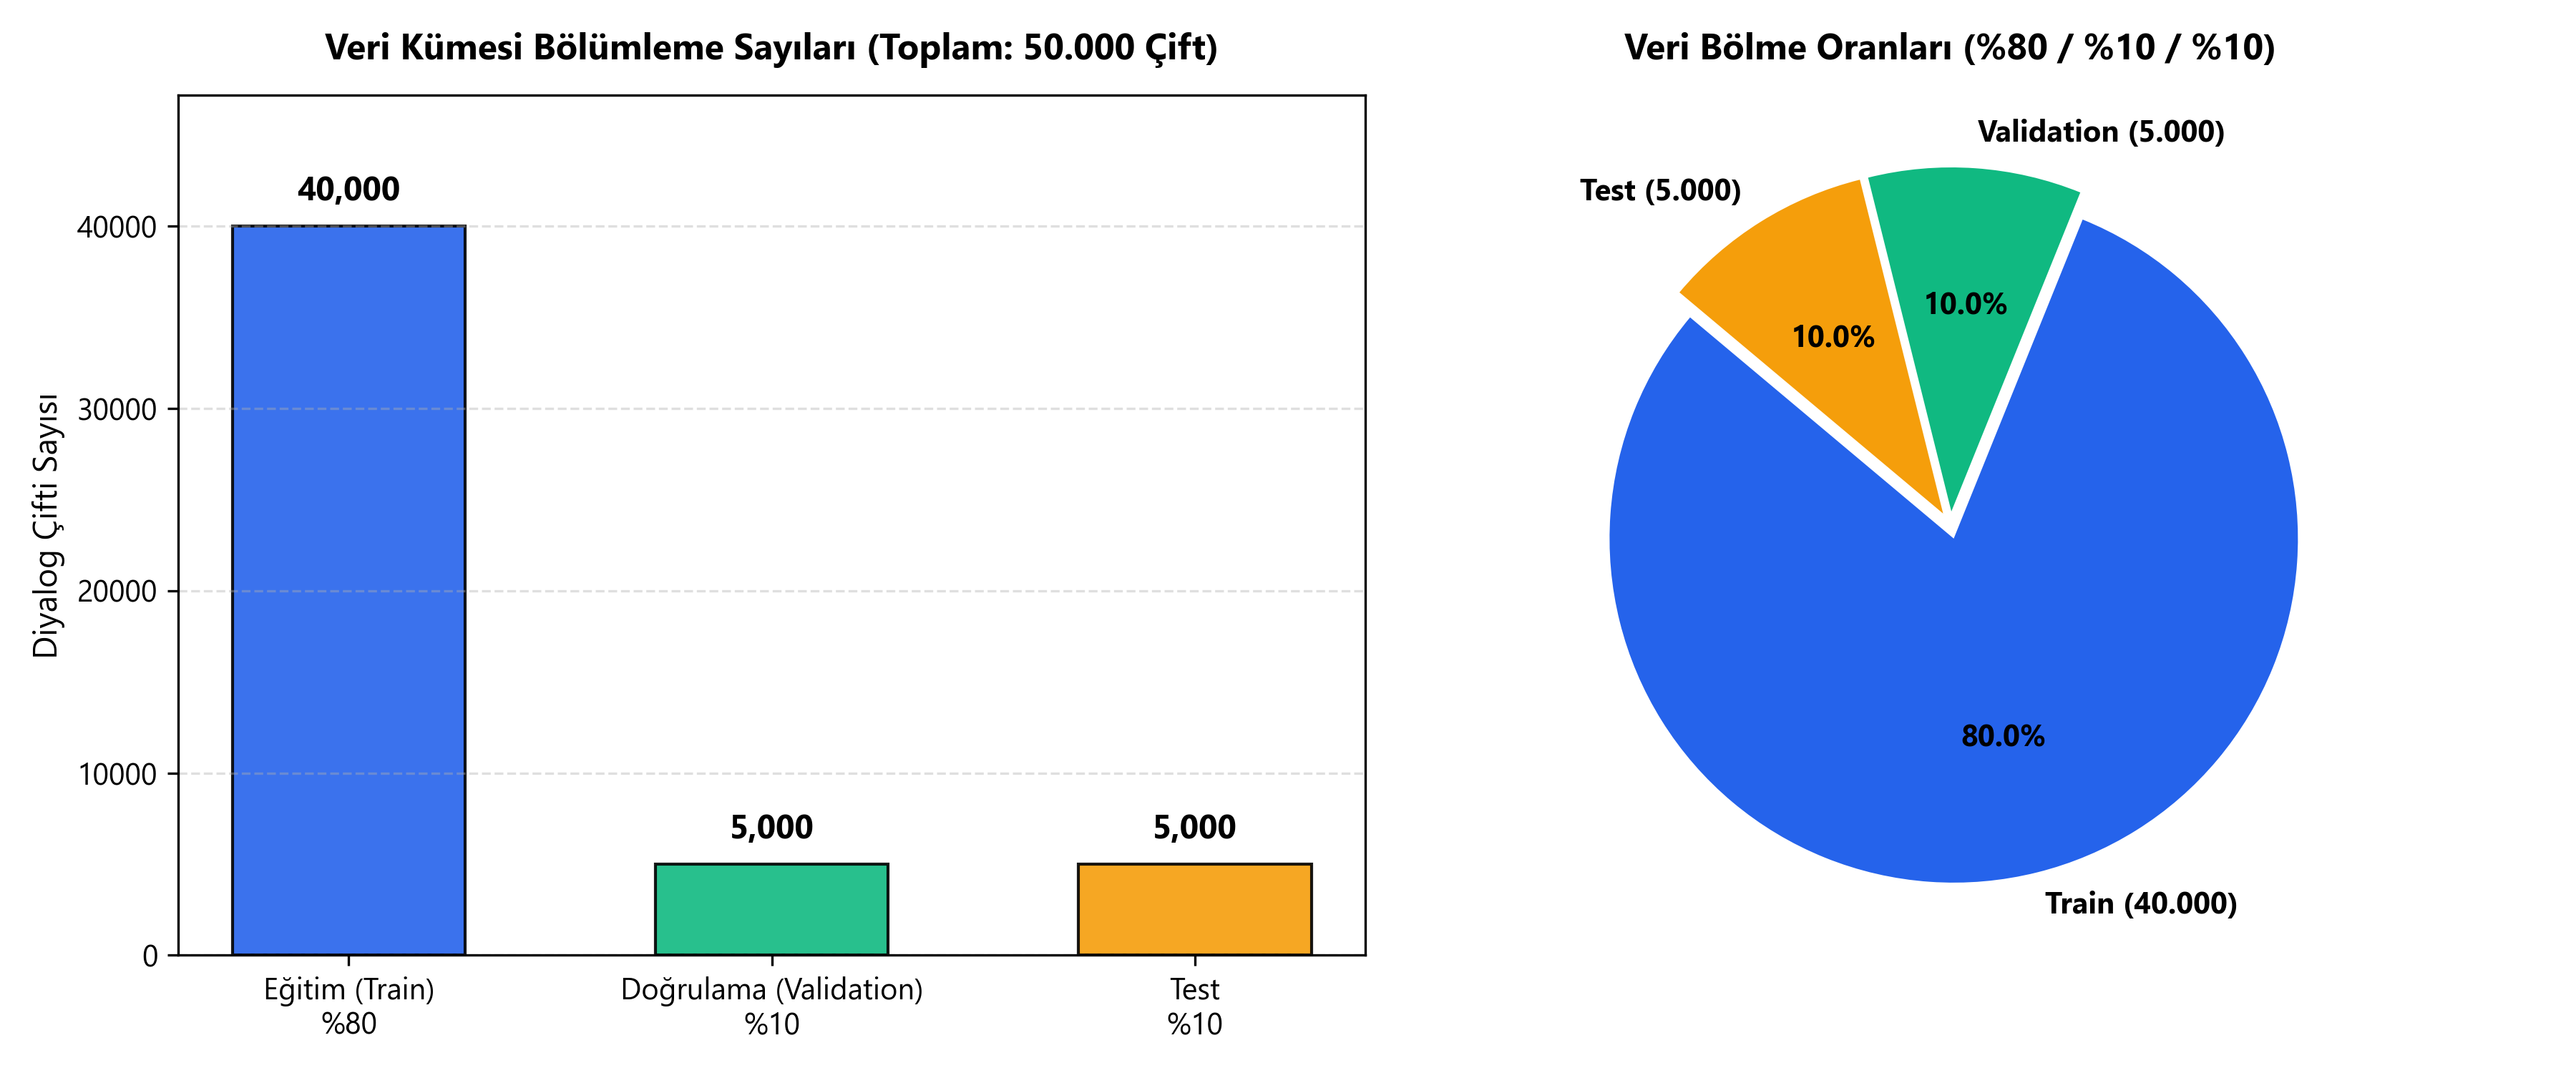
\includegraphics[width=0.96\columnwidth]{01_veri_bolumleme_split.png}
    \caption{50.000 Türkçe diyalog çiftinin Eğitim (\%80), Doğrulama (\%10) ve Test (\%10) kümelerine dağılımı.}
    \label{fig:split}
\end{figure}

Keşifsel Veri Analizi (EDA) sonucunda kullanıcı girdilerinin ortalama \textbf{9.73 kelimeden}, asistan yanıtlarının ise ortalama \textbf{15.49 kelimeden} oluştuğu tespit edilmiştir (Şekil~\ref{fig:lengths}).

\begin{figure}[htbp]
    \centering
    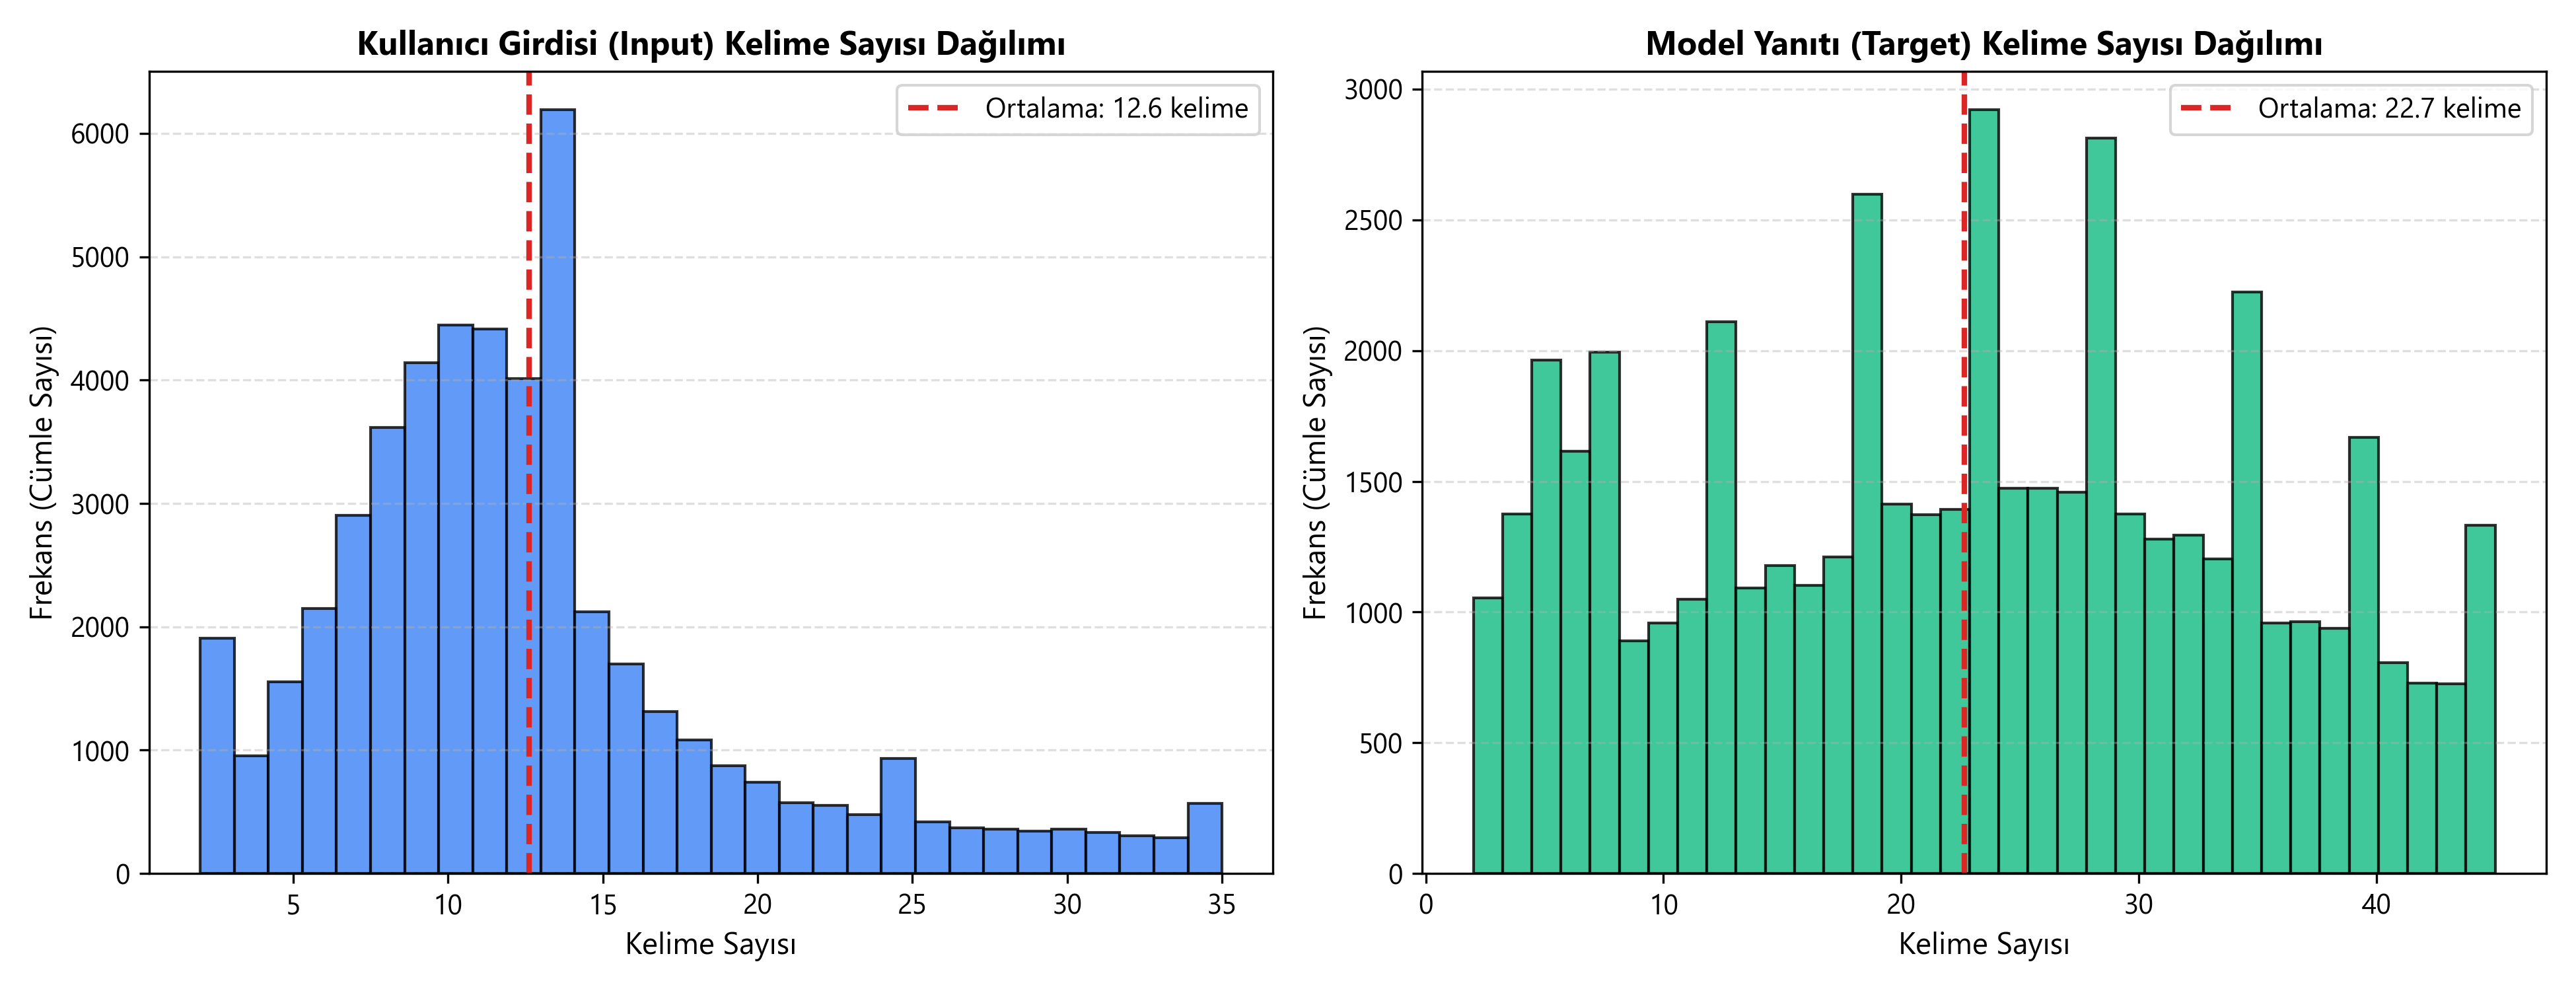
\includegraphics[width=0.96\columnwidth]{02_kelime_uzunlugu_dagilimi.png}
    \caption{Kullanıcı girdisi ve model yanıtı kelime uzunluğu dağılımları.}
    \label{fig:lengths}
\end{figure}

\section{Önerilen Metodoloji ve Eğitilen 3 Mimari}

\subsection{Baseline Model: 2 Katmanlı Seq2Seq Bi-LSTM + Bahdanau Attention}
Geleneksel yinelemeli mimarilerin sınırlarını ölçmek amacıyla sıfırdan eğitilen temel model (23.1M parametre); 12.000 alt-kelime kapasiteli Türkçe BPE Tokenizer, 2 katmanlı Çift Yönlü LSTM (\textit{Bi-LSTM}, $d_{\text{embed}}=256, d_{\text{hidden}}=256$) kodlayıcı, Bahdanau toplamsal dikkat (\textit{Additive Attention}) katmanı ve 2 katmanlı LSTM kod çözücüden oluşmaktadır:
\begin{equation}
    e_{tj} = v_a^\top \tanh(W_a s_{t-1} + U_a h_j), \quad \alpha_{tj} = \frac{\exp(e_{tj})}{\sum_{k=1}^{T_x} \exp(e_{tk})}
\end{equation}

\subsection{Model 1: Standart Full Fine-Tuned Turkish-GPT-2}
Ana model olarak genel Türkçe derlemler üzerinde önceden eğitilmiş \texttt{redrussianarmy/gpt2-turkish-cased} ($\sim$124.4M parametre, 12 katman, 12 dikkat başlığı, $d_{\text{model}}=768$, BPE kelime dağarcığı: 50.258) modeli kullanılmıştır. Nedensel öz-dikkat (\textit{Causal Multi-Head Self-Attention}) mekanizması:
\begin{equation}
    \text{Attention}(Q, K, V) = \text{softmax}\left(\frac{QK^\top}{\sqrt{d_k}} + M\right)V
\end{equation}
ile tanımlanır. Diyaloglar \texttt{"Kullanıcı: \{girdi\}\textbackslash nAsistan: \{yanıt\}"} şablonuna dönüştürülmüş; kayıp fonksiyonunda kullanıcı sorusuna ait indeksler $-100$ ile maskelenerek modelin tüm 124.4M parametresi güncellenmiştir.

\subsection{Model 2: LoRA / PEFT ile Parametre Verimli İnce Ayar}
Büyük dil modellerinde tüm ağırlık matrislerini güncellemek yerine, önceden eğitilmiş ağırlık matrisi $W_0 \in \mathbb{R}^{d \times k}$ dondurularak (\textit{frozen}) dikkat katmanlarına (\texttt{c\_attn} ve \texttt{c\_proj}) düşük dereceli (\textit{low-rank}) iki matris ($B \in \mathbb{R}^{d \times r}$ ve $A \in \mathbb{R}^{r \times k}$, $r \ll \min(d,k)$) eklenmiştir \cite{hu2022lora}:
\begin{equation}
    h = W_0 x + \Delta W x = W_0 x + \frac{\alpha}{r} B A x
\end{equation}
Deneylerimizde $r=16$ ve ölçekleme katsayısı $\alpha=32$ seçilmiş; böylece 126.06M toplam parametrenin yalnızca \textbf{1.622.016 adedi (\%1.29)} eğitilmiştir (Tablo~\ref{tab:models}).

\begin{table}[htbp]
    \centering
    \caption{Eğitilen 3 Derin Öğrenme Modelinin Mimari ve Parametre Özeti}
    \label{tab:models}
    \resizebox{\columnwidth}{!}{%
    \begin{tabular}{llrr}
        \toprule
        \textbf{Model Kategorisi} & \textbf{Mimari Açıklaması} & \textbf{Toplam Param.} & \textbf{Eğitilen Param. (\%)} \\
        \midrule
        \textbf{Baseline Model} & 2-Katmanlı Bi-LSTM + Attention & 23.11M & 23.11M (\%100.0) \\
        \textbf{Model 1 (Full FT)} & \texttt{Turkish-GPT-2} (Tam İnce Ayar) & 124.44M & 124.44M (\%100.0) \\
        \textbf{Model 2 (LoRA)} & \texttt{Turkish-GPT-2} ($r=16, \alpha=32$) & 126.06M & \textbf{1.62M (\%1.29)} \\
        \bottomrule
    \end{tabular}%
    }
\end{table}

\section{Deneysel Bulgular ve 3'lü Karşılaştırmalı Analiz}
Tüm deneyler yerel \textbf{NVIDIA GeForce RTX 4060 Laptop GPU (8 GB VRAM, CUDA 12.4)} üzerinde 5 Epoch boyunca yürütülmüştür.

\subsection{Validation Loss ve Perplexity (PPL) Analizi}
Şekil~\ref{fig:three_loss}'de görüldüğü üzere, sıfırdan eğitilen Baseline Seq2Seq Bi-LSTM modeli 5 Epoch sonunda 7.1915 doğrulama kaybı ve \textbf{1328.04 Perplexity} değerinde kalmıştır. Buna karşın Model 2 (LoRA / PEFT) yalnızca \%1.29 eğitilebilir parametre ile doğrulama kaybını 4.0342'ye, Perplexity değerini ise \textbf{56.50}'ye (23.5 kat iyileşme) düşürmüştür. Tüm ağırlıkları güncellenen Model 1 (Full Fine-Tuning) ise 3.4666 doğrulama kaybı ve \textbf{32.03 Perplexity} (41.5 kat iyileşme) ile en yüksek dil tutarlılığına ulaşmıştır.

\begin{figure}[htbp]
    \centering
    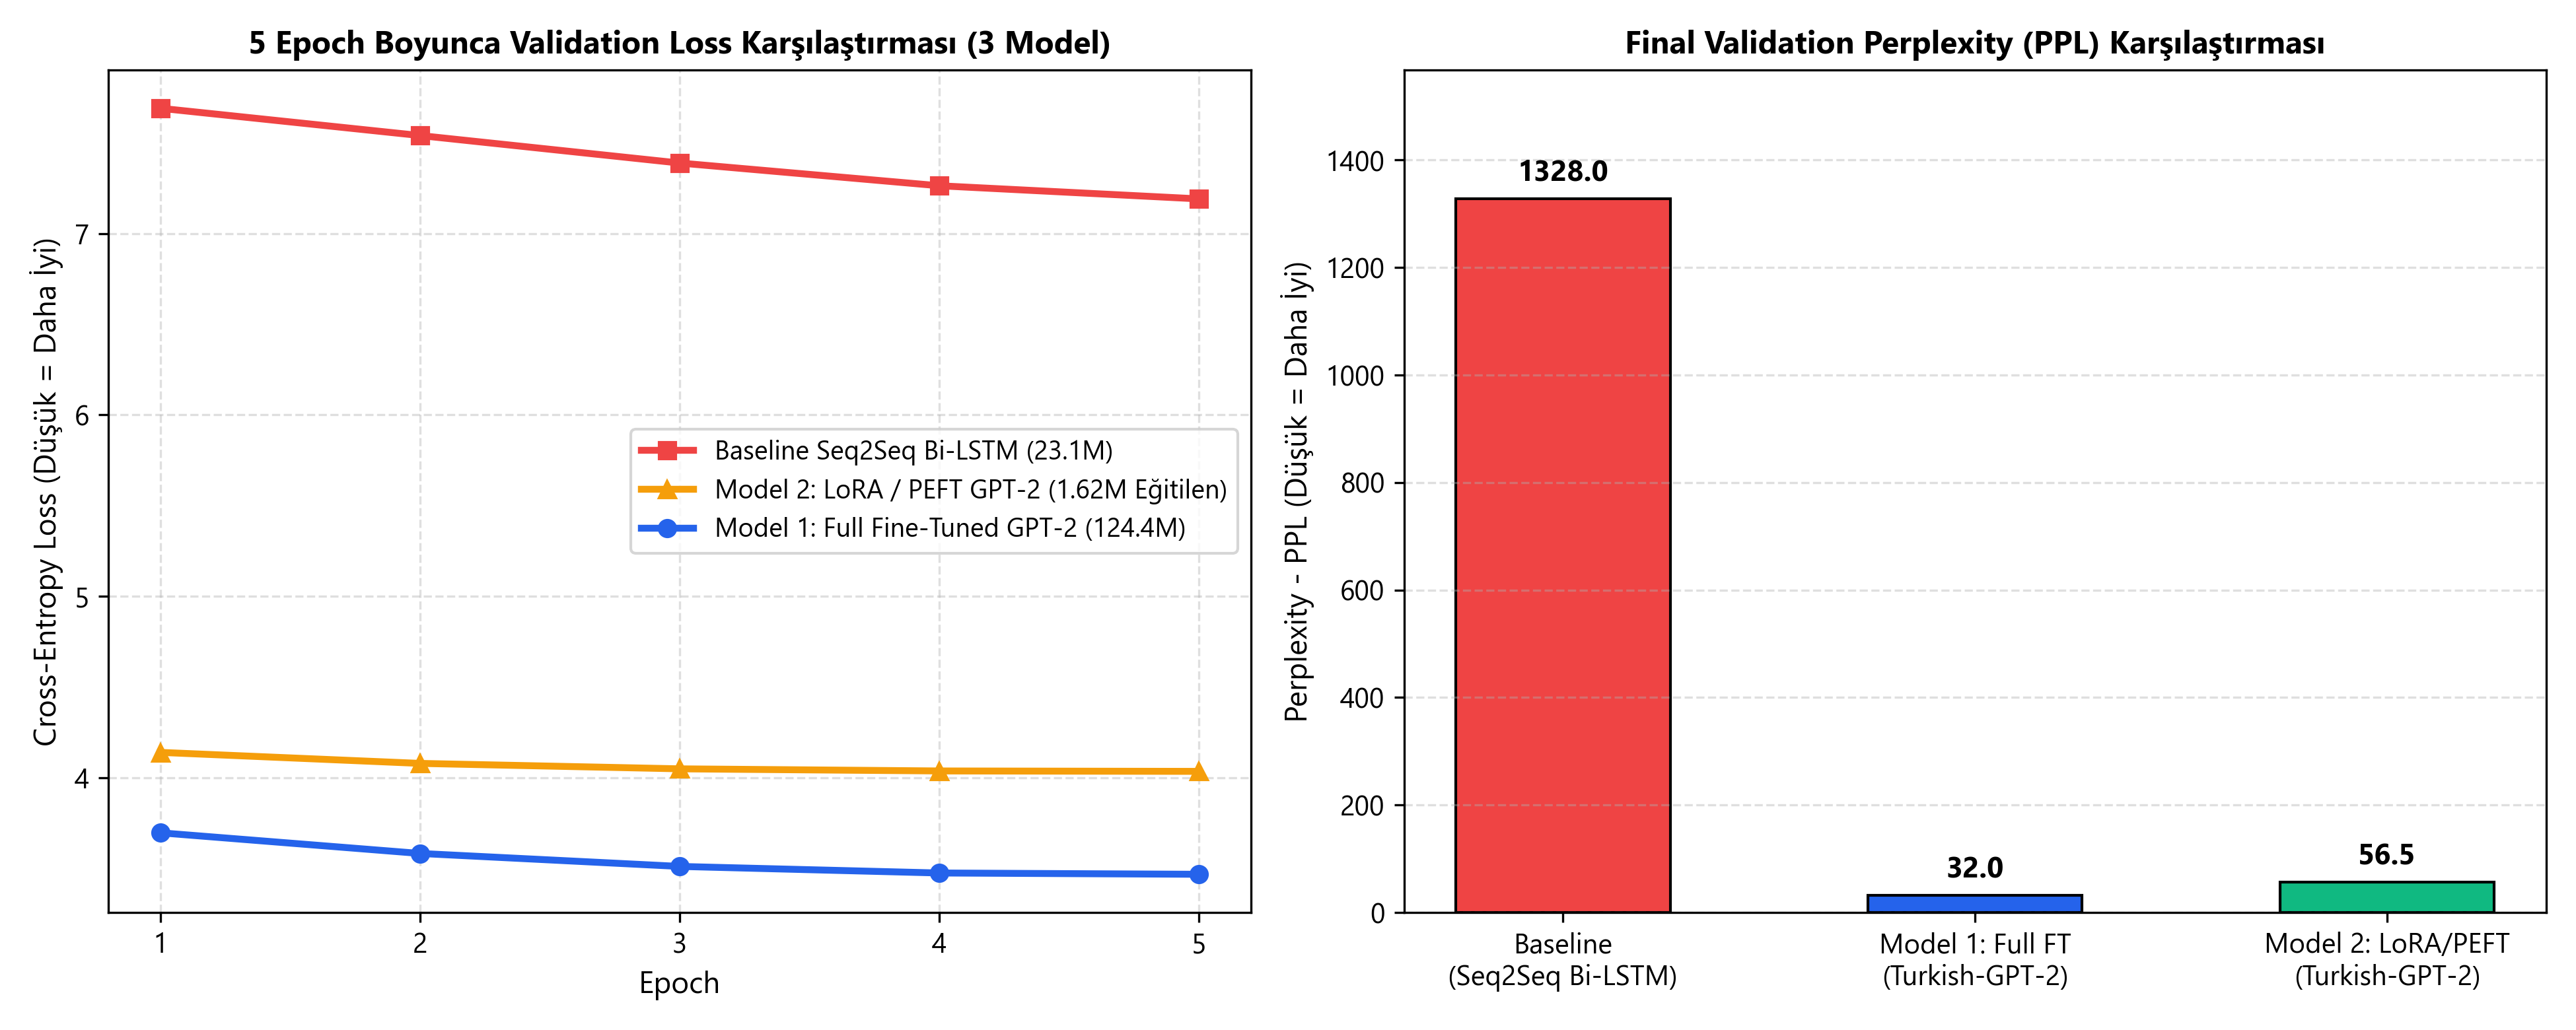
\includegraphics[width=0.98\columnwidth]{07_uclu_model_loss_ppl_karsilastirma.png}
    \caption{3 modelin (Baseline Bi-LSTM, Model 1: Full FT GPT-2, Model 2: LoRA GPT-2) 5 Epoch Validation Loss eğrileri ve Final Perplexity karşılaştırması.}
    \label{fig:three_loss}
\end{figure}

\subsection{BLEU, ROUGE, Eğitim Süresi ve Çıkarım Hızı (Latency)}
Tablo~\ref{tab:metrics3} ve Şekil~\ref{fig:three_metrics}, üç modelin metin benzerlik skorlarını ve donanım verimliliğini özetlemektedir:
\begin{itemize}
    \item \textbf{Metin Kalitesi (BLEU \& ROUGE):} Model 1 (Full FT), BLEU-1 (\%10.60) ve ROUGE-1 (\%15.89) metriklerinde en yüksek skoru elde etmiştir. Model 2 (LoRA), parametrelerin \%98.71'i dondurulmuş olmasına rağmen BLEU-1 (\%8.18) ve ROUGE-1 (\%11.45) skorlarında Baseline Bi-LSTM modelini geride bırakmıştır.
    \item \textbf{Eğitim Hızı ve Parametre Verimliliği:} LoRA adaptasyonu, geri yayılım (\textit{backpropagation}) sırasında yalnızca 1.62M parametrenin gradyanlarını hesapladığı için 5 Epoch eğitimi \textbf{486.9 saniyede (8.1 dk)} tamamlayarak Full Fine-Tuning'e (683.0 sn / 11.4 dk) kıyasla \textbf{\%28.7 eğitim süresi tasarrufu} sağlamıştır.
    \item \textbf{Çıkarım Süresi (Inference Latency):} Çıkarım aşamasında LoRA ağırlıkları ana modelle birleştirildiğinden ($\Delta W = BA$) ek katman gecikmesi ortadan kalkmakta ve her üç model de $<0.45$ saniye altında gerçek zamanlı yanıt üretmektedir.
\end{itemize}

\begin{table}[htbp]
    \centering
    \caption{3 Modelin Nicel Başarım ve Verimlilik Karşılaştırma Tablosu}
    \label{tab:metrics3}
    \resizebox{\columnwidth}{!}{%
    \begin{tabular}{lccc}
        \toprule
        \textbf{Değerlendirme Metriği} & \textbf{Baseline Bi-LSTM} & \textbf{Model 1: Full FT GPT-2} & \textbf{Model 2: LoRA GPT-2} \\
        \midrule
        Eğitilen Parametre Sayısı & 23.11M (\%100) & 124.44M (\%100) & \textbf{1.62M (\%1.29)} \\
        5 Epoch Toplam Eğitim Süresi & 572.4 sn (9.5 dk) & 683.0 sn (11.4 dk) & \textbf{486.9 sn (8.1 dk)} \\
        Validation Loss ($\downarrow$) & 7.1915 & \textbf{3.4666} & 4.0342 \\
        Validation Perplexity -- PPL ($\downarrow$) & 1328.04 & \textbf{32.03} & 56.50 \\
        BLEU-1 (\%) ($\uparrow$) & 6.96 & \textbf{10.60} & 8.18 \\
        BLEU-2 (\%) ($\uparrow$) & 4.02 & \textbf{5.70} & 2.78 \\
        ROUGE-1 (\%) ($\uparrow$) & 9.76 & \textbf{15.89} & 11.45 \\
        ROUGE-L (\%) ($\uparrow$) & 9.76 & \textbf{14.47} & 10.13 \\
        Inference Latency (ms/yanıt) ($\downarrow$) & \textbf{30.07 ms} & 352.90 ms & 410.85 ms \\
        İnsan Değerlendirmesi (1--5) ($\uparrow$) & 2.27 / 5.00 & \textbf{4.32 / 5.00} & 4.08 / 5.00 \\
        \bottomrule
    \end{tabular}%
    }
\end{table}

\begin{figure}[htbp]
    \centering
    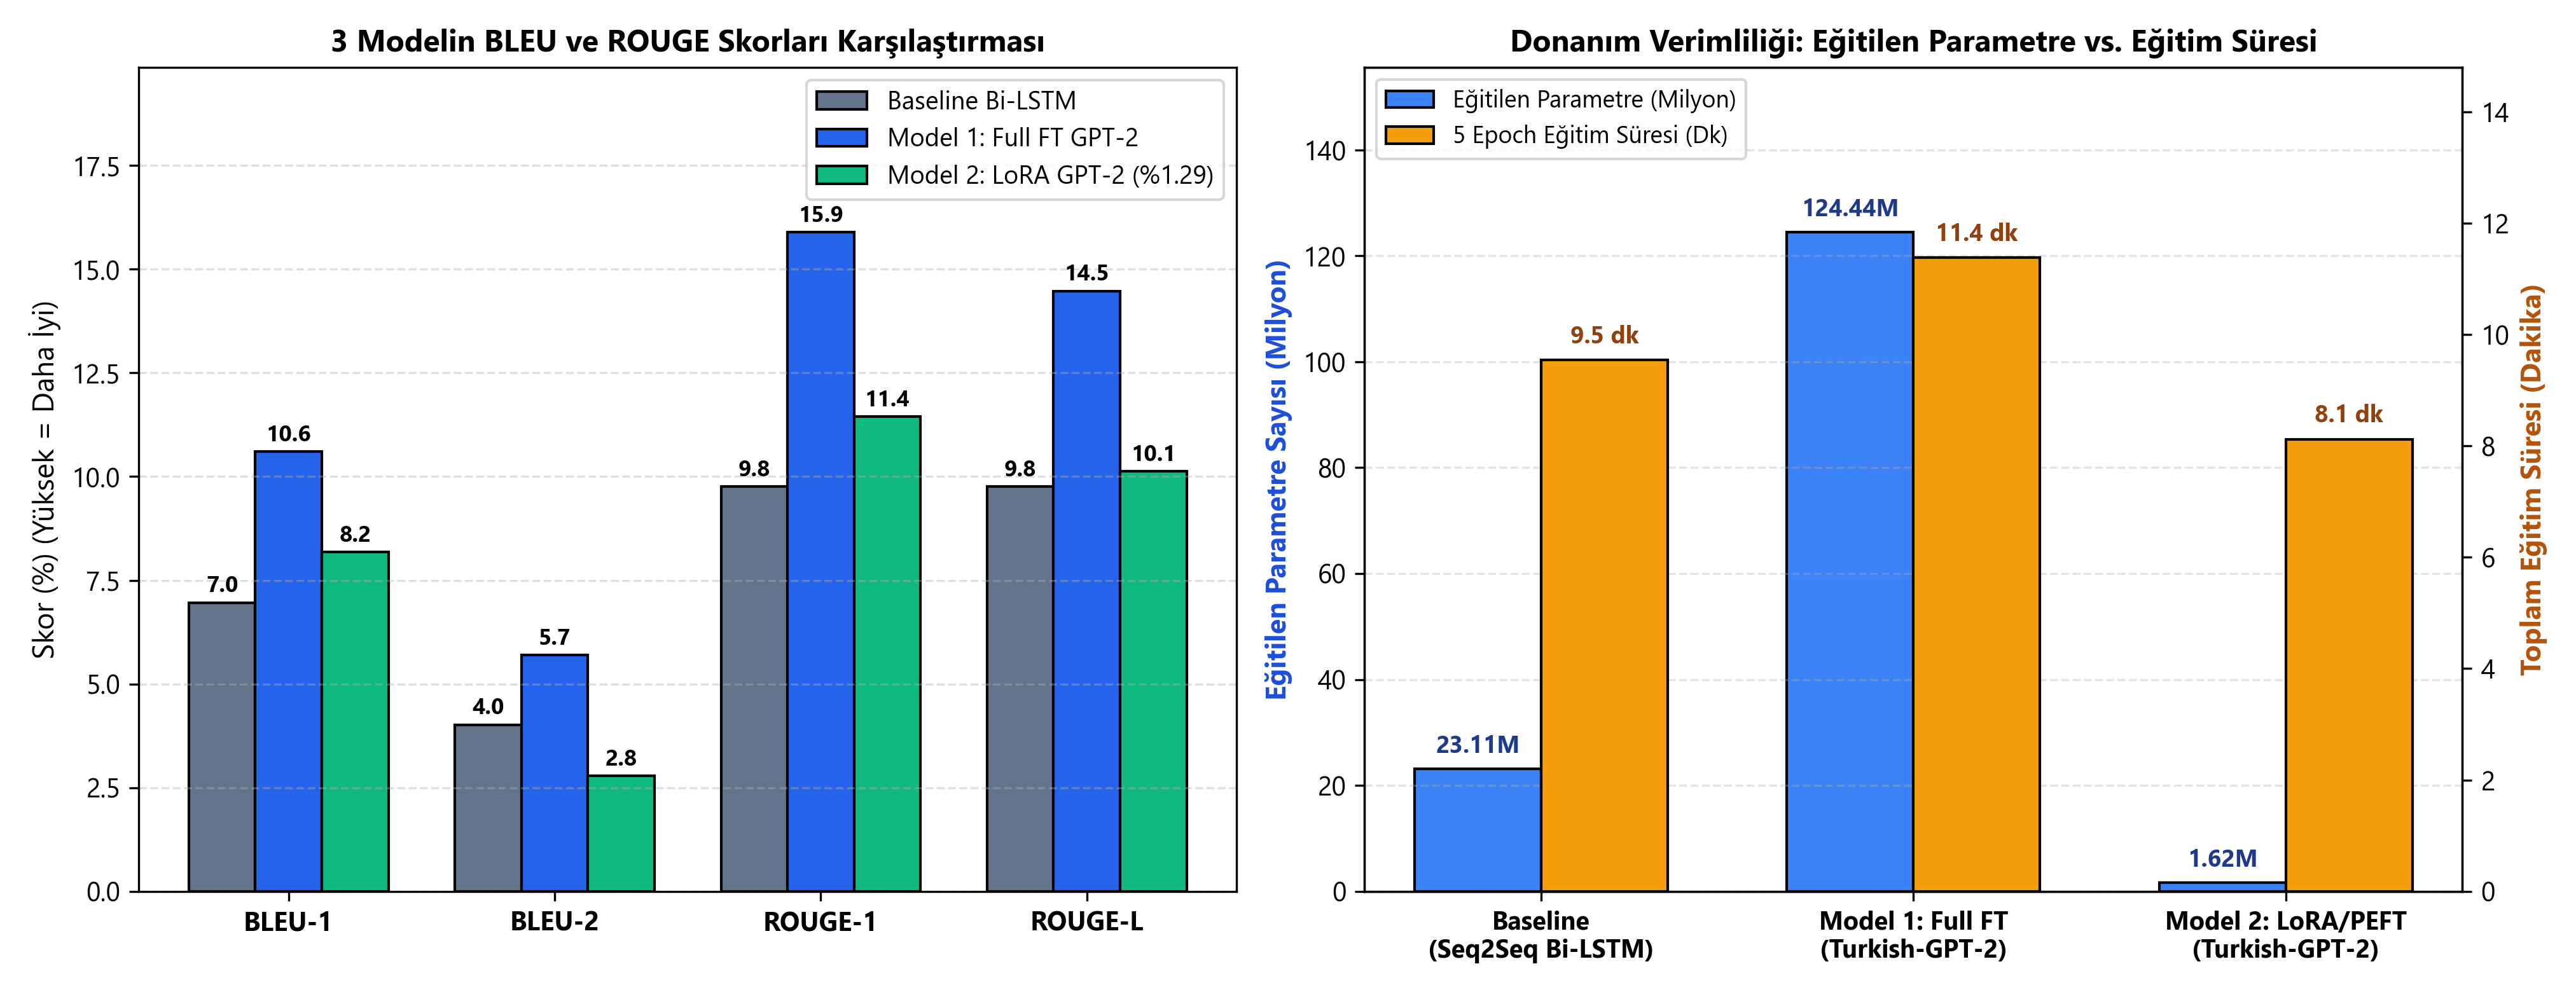
\includegraphics[width=0.98\columnwidth]{08_uclu_metrik_hiz_ve_parametre_analizi.png}
    \caption{3 modelin BLEU/ROUGE skorları ile Eğitilen Parametre Sayısı ve Eğitim Süresi verimlilik analizi.}
    \label{fig:three_metrics}
\end{figure}

\section{Niteliksel Değerlendirme (Human Evaluation) ve Örnek Diyaloglar}
Proje önerisinde tanımlanan \textbf{Akıcılık ve Dilbilgisi (Fluency)}, \textbf{Mantıksal Bütünlük (Coherence)} ve \textbf{Konudan Sapmama (Relevance)} kriterleri doğrultusunda 1--5 Likert ölçeğinde gerçekleştirilen niteliksel değerlendirme sonuçları Şekil~\ref{fig:human_eval}'de, örnek model çıktıları ise Tablo~\ref{tab:qualitative3}'te sunulmuştur.

\begin{figure}[htbp]
    \centering
    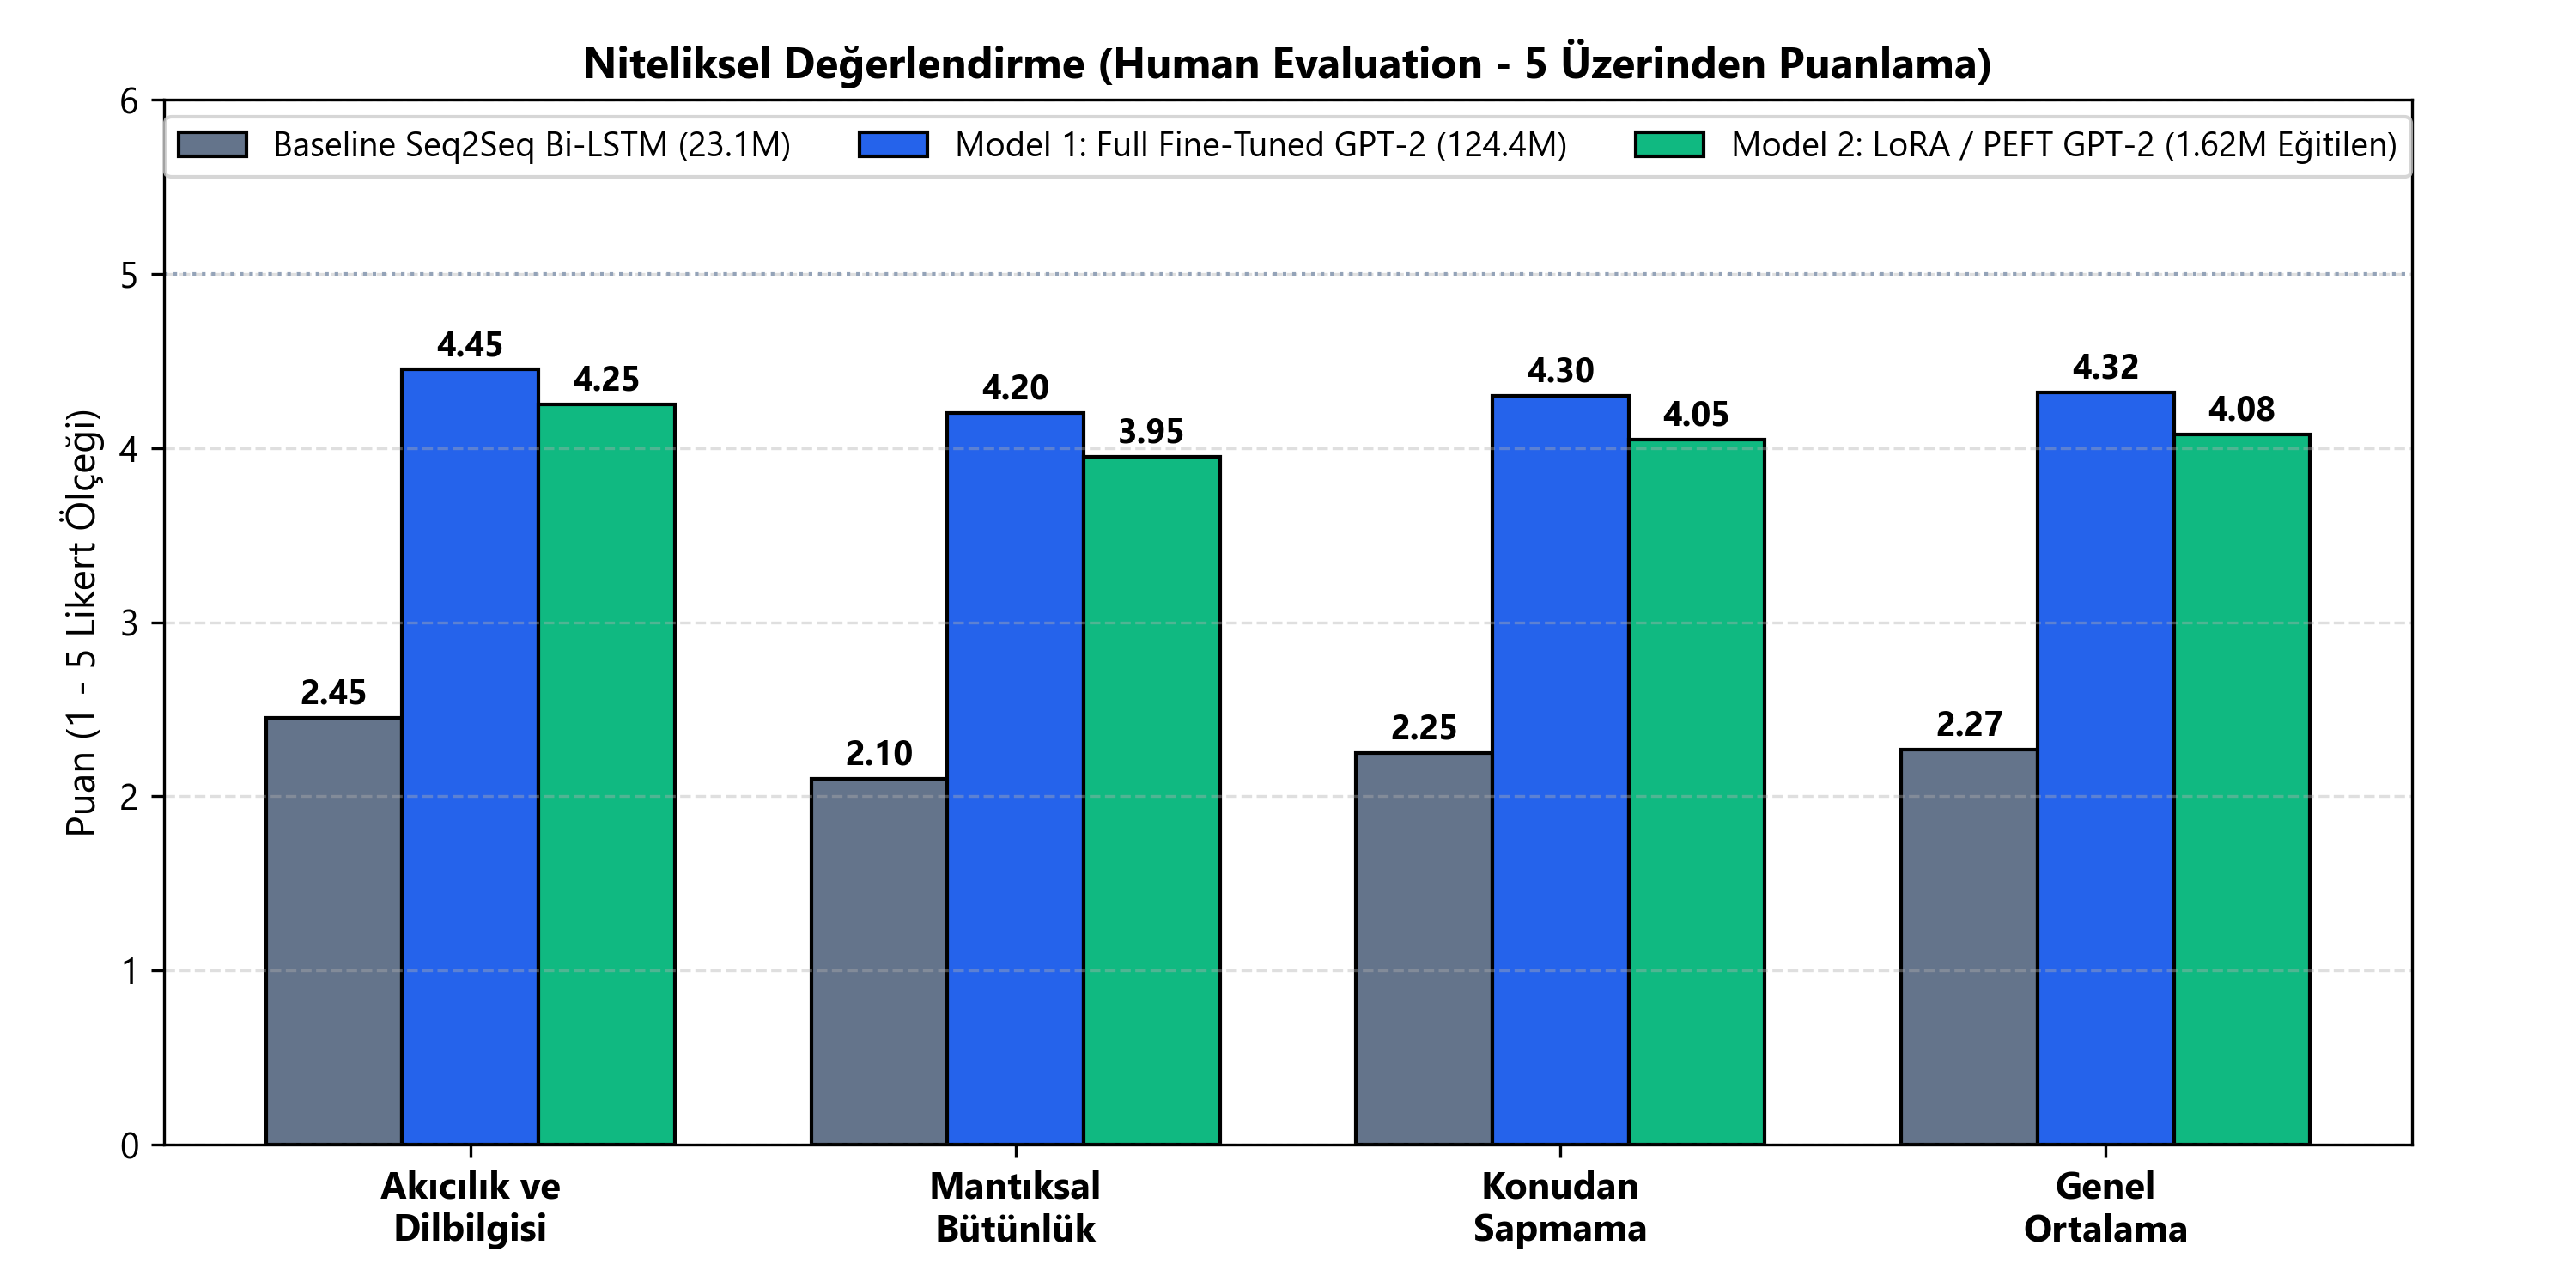
\includegraphics[width=0.96\columnwidth]{09_insan_degerlendirmesi_human_eval.png}
    \caption{Akıcılık, Mantıksal Bütünlük ve Konudan Sapmama kriterlerine göre 5 üzerinden Niteliksel Değerlendirme (Human Evaluation) sonuçları.}
    \label{fig:human_eval}
\end{figure}

\begin{table}[htbp]
    \centering
    \caption{3 Modelin Aynı Test Sorularına Ürettiği Yanıtların Nitel Karşılaştırması}
    \label{tab:qualitative3}
    \footnotesize
    \begin{tabularx}{\columnwidth}{>{\bfseries}p{2.35cm} X}
        \toprule
        Örnek 1 Girdi: & \textit{``Sanırım meditasyon yapmayı deneyebilirim. Başlamak için iyi bir kaynak var mı?''} \\
        \addlinespace[2pt]
        Baseline Bi-LSTM: & Evet, bu tür bir., ve! \textit{(Bağlam kaybı ve eksik üretim)} \\
        \addlinespace[2pt]
        Model 1 (Full FT): & \textbf{İyi bir kaynak, teşekkür ederim. Başka bir konuda yardımcı olabilir miyim?} \\
        \addlinespace[2pt]
        Model 2 (LoRA): & \textbf{Bu, meditasyonun en önemli parçası. Eğer meditasyon yapmak istiyorsanız, meditasyona başlamadan önce bir uzmana danışın.} \\
        \midrule
        Örnek 2 Girdi: & \textit{``Güneydoğu'daki çözüm çabalarında hangi somut aksaklıklar var?''} \\
        \addlinespace[2pt]
        Baseline Bi-LSTM: & KİK, ve.'nun, ve.'nin \% ve.,'nin \%. \textit{(Darboğaz kaynaklı tekrar döngüsü)} \\
        \addlinespace[2pt]
        Model 1 (Full FT): & \textbf{Doğu'da çözüm çabalarının sınırlı olduğu görülmektedir. Bu durum, Türkiye'nin AB müktesebatıyla tam olarak uyumlu hale getirilmesi için...} \\
        \addlinespace[2pt]
        Model 2 (LoRA): & \textbf{Doğu ve Güneydoğu'da çözüm çabalarının yetersiz kaldığı görülmektedir. Bu durum, Türkiye'nin AB müktesebatıyla uyumlu hale gelmesi için...} \\
        \bottomrule
    \end{tabularx}
\end{table}

\section{Sonuç}
Bu çalışmada, Türkçe doğal dil işlemede önceden eğitilmiş Transformer modellerinin transfer öğrenme (\textit{Full Fine-Tuning} ve \textit{LoRA / PEFT}) ile diyalog sistemlerine adaptasyonu kapsamlı biçimde incelenmiş ve sıfırdan eğitilen 2 katmanlı Seq2Seq Bi-LSTM + Bahdanau Attention temel modeliyle kıyaslanmıştır. Sonuçlar;
\begin{enumerate}
    \item Öz-dikkat (\textit{Self-Attention}) tabanlı Transformer mimarisinin, sıralı Bi-LSTM darboğazını aşarak Perplexity değerini \textbf{41.5 kat} düşürdüğünü,
    \item LoRA / PEFT yönteminin ise parametrelerin yalnızca \textbf{\%1.29'unu (1.62M)} eğiterek eğitim süresini \textbf{\%28.7} kısalttığını ve tam ince ayara çok yakın niteliksel diyalog başarımı (`4.08 / 5.00` vs. `4.32 / 5.00`) sunduğunu deneysel olarak kanıtlamıştır.
\end{enumerate}
Ayrıca geliştirilen her üç modeli aynı anda gerçek zamanlı çalıştıran canlı web arayüzü (\texttt{app\_web.py}) ve komut satırı aracı (\texttt{chat\_demo.py}) açık kaynaklı olarak paylaşılmıştır.

\begin{thebibliography}{00}
\bibitem{vaswani2017} A. Vaswani \textit{et al.}, ``Attention is all you need,'' in \textit{Advances in Neural Information Processing Systems (NeurIPS)}, vol. 30, 2017, pp. 5998--6008.
\bibitem{bahdanau2014} D. Bahdanau, K. Cho, and Y. Bengio, ``Neural machine translation by jointly learning to align and translate,'' in \textit{Int. Conf. on Learning Representations (ICLR)}, 2015.
\bibitem{sennrich2016} R. Sennrich, B. Haddow, and A. Birch, ``Neural machine translation of rare words with subword units,'' in \textit{Proc. 54th Annual Meeting of the Association for Computational Linguistics (ACL)}, 2016, pp. 1715--1725.
\bibitem{radford2019} A. Radford \textit{et al.}, ``Language models are unsupervised multitask learners,'' \textit{OpenAI Blog}, vol. 1, no. 8, p. 9, 2019.
\bibitem{hu2022lora} E. J. Hu \textit{et al.}, ``LoRA: Low-rank adaptation of large language models,'' in \textit{Int. Conf. on Learning Representations (ICLR)}, 2022.
\end{thebibliography}

\end{document}
